%!TEX root = ../../main.tex
\chapter{The Nonlinear Surface Susceptibility}\label{chap:chi2}
\partialtoc

In this section I will outline the general procedure to obtain the surface
susceptibility tensor for SHG. We start with the nonlinear polarization
$\mathbf{P}$ written as
\begin{equation}\label{mshg}
\begin{split}
P_{\mathrm{a}}(2\omega)
= \chi^{\mathrm{abc}}(-2\omega;\omega,\omega)
  E^{\mathrm{b}}(\omega)E^{\mathrm{c}}(\omega)
+ \chi^{\mathrm{abcd}}(-2\omega;\omega,\omega)
  E^{\mathrm{b}}(\omega)\nabla^{\mathrm{c}}E^{\mathrm{d}}(\omega)
+ \cdots,
\end{split}
\end{equation}
where $\chi^{\mathrm{abc}}(-2\omega;\omega,\omega)$ and
$\chi^{\mathrm{abcd}}(-2\omega;\omega,\omega)$ correspond to the dipolar and
quadrupolar susceptibilities. For ease of notation, I will drop the
$(-2\omega;\omega,\omega)$ argument from this point on. The sum continues with
higher multipolar terms. If we consider a semi-infinite system with a
centrosymmetric bulk, we can separate the terms into two contributions from
symmetry considerations alone. The first from the surface of the system, and the
second from the bulk of the system. We take
\begin{equation}\label{mshg2}
P^{\mathrm{a}}(\mathbf{r})
= \chi^{\mathrm{abc}}E^{\mathrm{b}}(\mathbf{r})E^{\mathrm{c}}(\mathbf{r})
+ \chi^{\mathrm{abcd}}E^{\mathrm{b}}(\mathbf{r})
  \frac{\partial}{\partial\mathbf{r}_{\mathrm{c}}}E^{\mathrm{d}}(\mathbf{r}) 
+ \cdots,
\end{equation}
as the polarization with respect to the original coordinate system, and 
\begin{equation}\label{mshg3}
P_{\mathrm{a}}(-\mathbf{r})
= \chi^{\mathrm{abc}}E^{\mathrm{b}}(-\mathbf{r})E^{\mathrm{c}}(-\mathbf{r})
+ \chi^{\mathrm{abcd}}E^{\mathrm{b}}(-\mathbf{r})
  \frac{\partial}{\partial(-\mathbf{r}_{\mathrm{c}})}E^{\mathrm{d}}(-\mathbf{r}) 
+ \cdots, 
\end{equation}
as the polarization in the coordinate system where inversion is taken, i.e.
$\mathbf{r} \rightarrow -\mathbf{r}$. Note that we have kept the same
susceptibility tensors as they must be invariant under $\mathbf{r} \to
-\mathbf{r}$ since the system is centrosymmetric. Recalling that
$\mathbf{P}(\mathbf{r})$ and $\mathbf{E}(\mathbf{r})$ are polar vectors
\cite{jacksonbook}, we have that Eq. \eqref{mshg3} reduces to
\begin{align}\label{mshg4}
-P^{\mathrm{a}}(\mathbf{r})
&= \chi^{\mathrm{abc}}(-E^{\mathrm{b}}(\mathbf{r}))(-E^{\mathrm{c}}(\mathbf{r}))
 + \chi^{\mathrm{abcd}}(-E^{\mathrm{b}}(\mathbf{r}))
(-\frac{\partial}{\partial\mathbf{r}_{\mathrm{c}}})(-E^{\mathrm{d}}(\mathbf{r})) 
 + \cdots,\nonumber\\
P^{\mathrm{a}}(\mathbf{r})
&= -\chi^{\mathrm{abc}}E^{\mathrm{b}}(\mathbf{r})E^{\mathrm{c}}(\mathbf{r})
 + \chi^{\mathrm{abcd}}E^{\mathrm{b}}(\mathbf{r})
   \frac{\partial}{\partial\mathbf{r}_{\mathrm{c}}}E^{\mathrm{d}}(\mathbf{r}) 
 + \cdots,
\end{align}
that when compared with Eq. \eqref{mshg2} leads to the conclusion that
\begin{equation}\label{sshg}
\chi^{\mathrm{abc}} = 0
\end{equation}
for a centrosymmetric bulk.

If we move to the surface of the semi-infinite system, our assumption of
centrosymmetry breaks down and there is no restriction on $\chi^{\mathrm{abc}}$.
We conclude that the leading term of the polarization in a surface region is
given by
\begin{equation}\label{sshgp1}
\int P^{\mathrm{a}}(\mathbf{R},z)\,dz \approx lP^{\mathrm{a}}
\equiv P^{\mathrm{a}}_{\mathrm{surface}}
\equiv \chi^{\mathrm{abc}}_{S}E^{\mathrm{b}}E^{\mathrm{c}},
\end{equation}
where $l$ is the surface region from which the dipolar signal of $\mathbf{P}$ is
different from zero (see Fig. \ref{fsystem}), and
$\mathbf{P}_{\mathrm{aurface}}\equiv l\mathbf{P}$ is the surface SH
polarization. Then, from Eq. \eqref{mshg} we obtain that
\begin{equation}\label{sshgp2}
\chi^{\mathrm{abc}}_{S} = l\chi^{\mathrm{abc}}
\end{equation}
is the SH surface susceptibility. On the other hand,
\begin{equation}\label{sshgp3}
P^{\mathrm{a}}_{\mathrm{bulk}}(\mathbf{r})
= \chi^{\mathrm{abcd}}
  E^{\mathrm{b}}(\mathbf{r})\nabla^{\mathrm{c}}E^{\mathrm{d}}(\mathbf{r}),  
\end{equation}
gives the bulk polarization. We immediately recognize that the surface
polarization is of dipolar order while the bulk polarization is of quadrupolar
order. The surface $\chi^{\mathrm{abc}}_{S}$, and bulk $\chi^{\mathrm{abcd}}$,
susceptibility tensor ranks are three and four, respectively. We will only
concentrate on SSHG in this work, even though bulk-generated SH is also a very
important optical phenomenon. I will also exclude other interesting surface SH
phenomena like, electric field induced second-harmonic (EFISH), which would be
represented by a surface susceptibility tensor of quadrupolar origin. As I
mentioned in Chapter \ref{chap:intro}, in centrosymmetric systems for which the
quadrupolar bulk response is much smaller than the dipolar surface response, SH
is a very capable and powerful optical surface probe \cite{downerSIA01}.

In the following sections of this chapter, we will review the theoretical
approach to derive the expressions for the surface susceptibility tensor
$\chi^{\mathrm{abc}}_{S}$.

\begin{figure}[t]
\centering
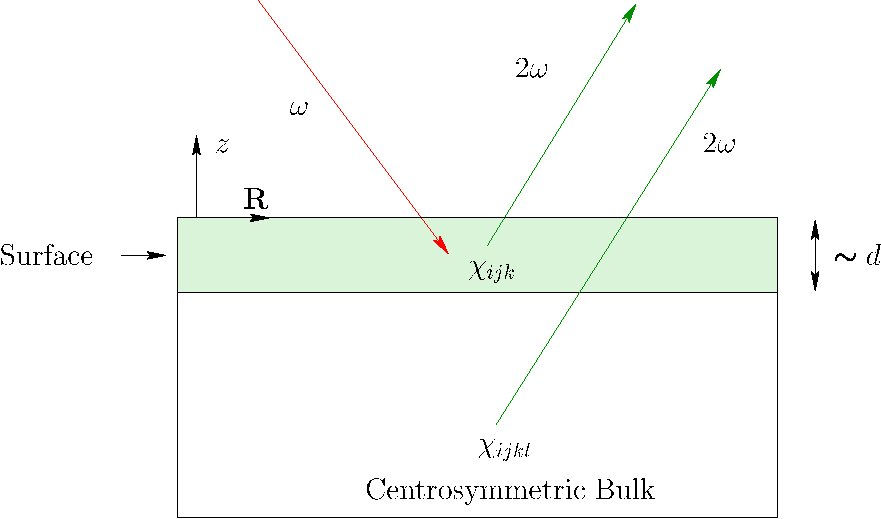
\includegraphics[scale=0.6]{content/figures/diag-system}
\caption{Sketch of a semi-infinite system with a centrosymmetric bulk. The
surface region is of width $\sim l$. The incoming photon of frequency $\omega$
is represented by a downward red arrow, whereas both the surface and bulk
created second-harmonic photons of frequency $2\omega$ are represented by upward
green arrows. The red color suggests an incoming infrared photon with a green
second-harmonic photon. The dipolar ($\chi^{\mathrm{abc}}$), and quadrupolar
($\chi^{\mathrm{abcd}}$) susceptibility tensors are shown in the regions where
they are nonzero. The $z$-axis is perpendicular to the surface and $\mathbf{R}$
is parallel to it.}
\label{fsystem}
\end{figure}


%%%%%%%%%%%%%%%%%%%%%%%%%%%%%%%%%%%%%%%%%%%%%%%%%%%%%%%%%%%%%%%%%%%%%%%%%%%%%%%%
%%%%%%%%%%%%%%%%%%%%%%%%%%%%%%%%%%%%%%%%%%%%%%%%%%%%%%%%%%%%%%%%%%%%%%%%%%%%%%%%

\section{Length Gauge}\label{longi}

We follow the article by Aversa and Sipe \cite{aversaPRB95} to calculate the
optical properties of a given system within the longitudinal gauge. More recent
derivations can also be found in Refs. \cite{sipePRB00} and
\cite{lambrechtPSSB00}. We assume the long-wavelength approximation which implies
a position independent electric field, $\mathbf{E}(t)$. The Hamiltonian in the
length gauge approximation is given by
\begin{equation}\label{ache}
\hat{H}=\hat{H}^{\Sigma}_{0} - e\hat{\mathbf{r}}\cdot\mathbf{E},
\end{equation}
with
\begin{align}\label{ache.1}
  \hat{H}^{\Sigma}_{0} = \hat{H}^{\mathrm{LDA}}_{0}
+ \mathcal{S}(\mathbf{r},\mathbf{p}),
\end{align} 
as the unperturbed Hamiltonian. The LDA Hamiltonian can be expressed as follows,
\begin{align}\label{ache.2}
\hat{H}^{\mathrm{LDA}}_{0}
&= \frac{\hat{p}^{2}}{2m_{e}} + \hat{V}^{\mathrm{ps}},\nonumber\\
\hat{V}^{\mathrm{ps}}
&= \hat{V}^{\mathrm{l}}(\hat{\mathbf{r}}) + \hat{V}^{\mathrm{nl}},
\end{align}  
where $\hat{V}^{\mathrm{l}}(\hat{\mathbf{r}})$ and $\hat{V}^{\mathrm{nl}}$ are
the local and the nonlocal parts of the crystal pseudopotential
$\hat{V}^{\mathrm{ps}}$. For the latter, we have that
\begin{align}\label{ache.3n}
V^{\mathrm{nl}}(\mathbf{r},\mathbf{r}')\equiv
\langle\mathbf{r}\vert
\hat{V}^{\mathrm{nl}}
\vert\mathbf{r}'\rangle \neq 0 
\quad\text{for}\quad\mathbf{r} \neq \mathbf{r}',
\end{align}
where $V^{\mathrm{nl}}(\mathbf{r},\mathbf{r}')$ is a function of $\mathbf{r}$
and $\mathbf{r}'$ representing the nonlocal contribution of the pseudopotential.
The Schr\"odinger equation reads
\begin{align}\label{ache.4} 
\left(
\frac{-\hbar^2}{2m_{e}}\nabla^{2}
+ \hat{V}^l(\mathbf{r})
\right)
\psi_{n\mathbf{k}}(\mathbf{r})
+ \int\hat{V}^{\mathrm{nl}}(\mathbf{r},\mathbf{r}')
  \psi_{n\mathbf{k}}(\mathbf{r}')\,d\mathbf{r}'
= E_{i}\psi_{n\mathbf{k}}(\mathbf{r}),
\end{align} 
where $\psi_{n\mathbf{k}}(\mathbf{r}) = \langle\mathbf{r}|n\mathbf{k}\rangle =
e^{i\mathbf{k}\cdot\mathbf{r}}u_{n\mathbf{k}}(\mathbf{r})$, are the real space
representations of the Bloch states $|n\mathbf{k}\rangle$ labeled by the band
index $n$ and the crystal momentum $\mathbf{k}$, and
$u_{n\mathbf{k}}(\mathbf{r})$ is cell periodic. $m_{e}$ is the bare mass of the
electron. The nonlocal scissors operator is given by
\begin{equation}\label{chon.0}
\mathcal{S}(\mathbf{r},\mathbf{p}) = 
\hbar\Delta\sum_{n}
\int(1 - f_{n}(\mathbf{k}))\vert n\mathbf{k}'\rangle \langle n\mathbf{k}'\vert
\,d^{3}k',
\end{equation}
where $f_{n}(\mathbf{k})$ is the occupation number that is independent of
$\mathbf{k}$ for $T = 0$ K, and is $f_{n} = 1$ for filled bands and $f_{n} = 0$
for unoccupied bands. For semiconductors the filled bands correspond to valence
bands ($n = v$), and unoccupied bands correspond to conduction bands ($n = c$).
We have that
\begin{equation}\label{chon.1}
\begin{split}
H^\mathrm{LDA}_{0}\vert n\mathbf{k}\rangle
    &= \hbar\omega^{\mathrm{LDA}}_{n}(\mathbf{k})\vert n\mathbf{k}\rangle\\
H^{\Sigma}_{0}\vert n\mathbf{k}\rangle
    &= \hbar\omega^{\Sigma}_{n}(\mathbf{k})\vert n\mathbf{k}\rangle,
\end{split}
\end{equation} 
where 
\begin{equation}\label{chon.78}
\hbar\omega^{\Sigma}_{n}(\mathbf{k})
= \hbar\omega^{\mathrm{LDA}}_{n}(\mathbf{k}) + \hbar\Delta(1 - f_{n}),
\end{equation}
is the scissored energy. Here, $\hbar\Delta$ is the value by which the
conduction bands are rigidly ($\mathbf{k}$-independent) shifted upwards in
energy, also known as the scissors shift. $\Delta$ could be taken to be
$\mathbf{k}$ dependent, but for most calculations (like the ones presented
here), a rigid shift is sufficient. We can take $\hbar\Delta = E_{g} -
E_{g}^\mathrm{LDA}$ where $E_{g}$ is the experimental or GW band gap taken at
the $\Gamma$ point, i.e. $\mathbf{k} = 0$. We used the fact that $\vert
n\mathbf{k}\rangle^\mathrm{LDA} \approx \vert n\mathbf{k}\rangle^\Sigma$, thus
negating the need to label the Bloch states with the LDA or $\Sigma$
superscripts. The matrix elements of $\mathbf{r}$ are split between the
\emph{intraband} ($\mathbf{r}_{i}$) and \emph{interband} ($\mathbf{r}_{e}$)
parts, where $\mathbf{r} = \mathbf{r}_{i} + \mathbf{r}_{e}$
\cite{adamsJCP53, blountSSP62, aversaPRB95} and
\begin{align}\label{rnminn}
\langle n\mathbf{k}\vert \hat{\mathbf{r}}_{i} |m\mathbf{k}'\rangle 
&= \delta_{nm}
\left[
  \delta(\mathbf{k} - \mathbf{k}')\boldsymbol{\xi}_{nn}(\mathbf{k})
+ i\nabla_{\mathbf{k}}\delta(\mathbf{k} - \mathbf{k}')
\right],\\
\langle n\mathbf{k}| \hat{\mathbf{r}}_{e} |m\mathbf{k}'\rangle 
&= (1- \delta_{nm})\delta(\mathbf{k}-\mathbf{k}')
   \boldsymbol{\xi}_{nm}(\mathbf{k}),\label{rnmenn}
\end{align}
with
\begin{equation}\label{zetann}
\boldsymbol{\xi}_{nm}(\mathbf{k})
\equiv i\frac{(2\pi)^3}{\Omega}
\int_{\Omega}u^{*}_{n\mathbf{k}}(\mathbf{r})
\nabla_{\mathbf{k}}\,u_{m\mathbf{k}}(\mathbf{r})
\,d\mathbf{r},
\end{equation}
where $\Omega$ is the unit cell volume. The interband part, $\mathbf{r}_{e}$,
can be obtained as follows. We start by introducing the velocity operator
\begin{align}\label{vop}
\hat{\mathbf{v}}^{\Sigma} &=
\frac{1}{i\hbar}\left[\hat{\mathbf{r}},\hat{H}^{\Sigma}_{0}\right],
\end{align}
and calculating its matrix elements
\begin{equation}\label{conhrnm}
i\hbar\langle n\mathbf{k}\vert\mathbf{v}^\Sigma\vert m\mathbf{k}\rangle
= \langle n\mathbf{k}\vert
\left[
\hat{\mathbf{r}}, \hat{H}^{\Sigma}_{0}
\right]
  \vert m\mathbf{k}\rangle
= \langle n\mathbf{k}\vert
\hat{\mathbf{r}}\hat{H}^{\Sigma}_{0} - \hat{H}^{\Sigma}_{0}\hat{\mathbf{r}}
\vert m\mathbf{k}\rangle
=
\left(
\hbar\omega^{\Sigma}_{m}(\mathbf{k}) - \hbar\omega^{\Sigma}_{n}(\mathbf{k})
\right)
\langle n\mathbf{k}\vert\hat{\mathbf{r}}\vert m\mathbf{k}\rangle.
\end{equation}
Defining $\omega^\Sigma_{nm}(\mathbf{k}) =
\omega^{\Sigma}_{n}(\mathbf{k}) - \omega^\Sigma_m(\mathbf{k})$, we get
\begin{equation}\label{pmnrmn}
\mathbf{r}_{nm}(\mathbf{k})
= \frac{\mathbf{v}^\Sigma_{nm}(\mathbf{k})}{i\omega^\Sigma_{nm}(\mathbf{k})}
\qquad n\notin D_{m},
\end{equation} 
which can be identified as
$\mathbf{r}_{nm}=(1-\delta_{nm})\boldsymbol{\xi}_{nm}\to \mathbf{r}_{e,nm}$.
Here, $D_m$ are all the possible degenerate $m$-states. When $\mathbf{r}_{i}$
appears in commutators we use \cite{aversaPRB95}
\begin{equation}\label{conmri3n}
\langle n\mathbf{k}\vert
\left[
\hat{\mathbf{r}}_{i}, \hat{\mathcal{O}}
\right]
\vert m\mathbf{k}'\rangle
= i\delta(\mathbf{k} - \mathbf{k}')(\mathcal{O}_{nm})_{;\mathbf{k}},
\end{equation}  
with
\begin{equation}\label{gendevnn}
(\mathcal{O}_{nm})_{;\mathbf{k}} =
  \nabla_{\mathbf{k}}\mathcal{O}_{nm}(\mathbf{k})
- i\mathcal{O}_{nm}(\mathbf{k})
\left(
\boldsymbol{\xi}_{nn}(\mathbf{k}) - \boldsymbol{\xi}_{mm}(\mathbf{k})
\right),
\end{equation} 
where ``$;\mathbf{k}$'' denotes the generalized derivative (see Appendix
\ref{app:re_ri}).

As can be seen from Eq. \eqref{ache.1} and \eqref{ache.2}, both $\mathcal{S}$
and $\hat{V}^{\mathrm{nl}}$ are nonlocal potentials. Their contribution in the
calculation of the optical response has to be considered in order to get
reliable results \cite{ismailPRL01}. We proceed as follows: from Eqs.
\eqref{vop}, \eqref{ache.1} and \eqref{ache.2} we find
\begin{align}\label{vop2}
\hat{\mathbf{v}}^{\Sigma} &=
\frac{\hat{\mathbf{p}}}{m_{e}} + \frac{1}{i\hbar}
\left[\hat{\mathbf{r}},\hat{V}^{\mathrm{nl}}(\mathbf{r},\mathbf{r}')\right]
+ \frac{1}{i\hbar}
  \left[\hat{\mathbf{r}},\hat{\mathcal{S}}(\mathbf{r},\mathbf{p})\right]
\nonumber\\
&\equiv
\hat{\mathbf{v}} + \hat{\mathbf{v}}^{\mathrm{nl}} + \hat{\mathbf{v}}^\mathcal{S}
= \hat{\mathbf{v}}^\mathrm{LDA} + \hat{\mathbf{v}}^\mathcal{S},
\end{align}
where we have defined
\begin{equation}\label{conhr}
\begin{split}
\hat{\mathbf{v}} &=\frac{\hat{\mathbf{p}}}{m_{e}}\\
\hat{\mathbf{v}}^{\mathrm{nl}} &= \frac{1}{i\hbar}
  \left[\hat{\mathbf{r}},\hat{V}^{\mathrm{nl}}\right]\\
\hat{\mathbf{v}}^\mathcal{S} &= \frac{1}{i\hbar}
  \left[\hat{\mathbf{r}},\hat{S}(\mathbf{r},\mathbf{p})\right]\\
\hat{\mathbf{v}}^\mathrm{LDA} &= \hat{\mathbf{v}}+\hat{\mathbf{v}}^{\mathrm{nl}}
\end{split}
\end{equation}  
with $\hat{\mathbf{p}}= -i\hbar\boldsymbol{\nabla}$ the momentum operator. Using
Eq. \eqref{chon.0}, we obtain that the matrix elements of
$\hat{\mathbf{v}}^\mathcal{S}$ are given by
\begin{equation}\label{chon.2} 
\mathbf{v}^\mathcal{S}_{nm} = i\Delta f_{mn}\mathbf{r}_{nm},
\end{equation}
with $f_{nm} = f_{n} - f_{m}$, where we see that $\mathbf{v}^\mathcal{S}_{nn} =
0$, then
\begin{align}\label{chon.8}
\mathbf{v}^\Sigma_{nm} 
&= \mathbf{v}^\mathrm{LDA}_{nm} + i\Delta f_{mn}\mathbf{r}_{nm}\nonumber\\
&= \mathbf{v}^\mathrm{LDA}_{nm} + i\Delta f_{mn}
   \frac{\mathbf{v}^\Sigma_{nm}(\mathbf{k})}{i\omega^\Sigma_{nm}(\mathbf{k})}
   \nonumber\\
%%%%%%%%%%%%%%%%%%%%%%%%%%%%%%%%%%%%%%%%%%%%%%%%%
\mathbf{v}^\Sigma_{nm}
  \frac{\omega^\Sigma_{nm}-\Delta f_{mn}}{\omega^\Sigma_{nm}}
&= \mathbf{v}^\mathrm{LDA}_{nm}\nonumber\\
%%%%%%%%%%%%%%%%%%%%%%%%%%%%%%%%%%%%%%%%%%%%%%%%%
\mathbf{v}^\Sigma_{nm}\frac{\omega^{\mathrm{LDA}}_{nm}}{\omega^\Sigma_{nm}}
&= \mathbf{v}^\mathrm{LDA}_{nm}\nonumber\\
%%%%%%%%%%%%%%%%%%%%%%%%%%%%%%%%%%%%%%%%%%%%%%%%%
\frac{\mathbf{v}^\Sigma_{nm}}{\omega^\Sigma_{nm}}
&= \frac{\mathbf{v}^\mathrm{LDA}_{nm}}{\omega^{\mathrm{LDA}}_{nm}},
\end{align}
since $\omega^\Sigma_{nm}-\Delta f_{mn}=\omega^{\mathrm{LDA}}_{nm}$. Therefore,
\begin{align}\label{chon.9}
\begin{split}
\mathbf{v}^\Sigma_{nm}(\mathbf{k}) &=
\frac{\omega^\Sigma_{nm}}{\omega^{\mathrm{LDA}}_{nm}}
\mathbf{v}^\mathrm{LDA}_{nm}(\mathbf{k})
= \left(
1 + \frac{\Delta}{\omega_c(\mathbf{k})-\omega_v(\mathbf{k})}
\right)
\mathbf{v}^\mathrm{LDA}_{nm}(\mathbf{k})\qquad n\notin D_{m}\\\\
\mathbf{v}^\Sigma_{nn}(\mathbf{k}) &= \mathbf{v}^\mathrm{LDA}_{nn}(\mathbf{k}),
\end{split}
\end{align} 
and Eq. \eqref{pmnrmn} gives
\begin{align}\label{chon.10}
\mathbf{r}_{nm}(\mathbf{k})
= \frac{\mathbf{v}^\Sigma_{nm}(\mathbf{k})}{i\omega^\Sigma_{nm}(\mathbf{k})}
= \frac{\mathbf{v}^\mathrm{LDA}_{nm}(\mathbf{k})}
{i\omega^{\mathrm{LDA}}_{nm}(\mathbf{k})} \qquad n\notin D_{m}.
\end{align}
The matrix elements of $\mathbf{r}_{e}$ are the same whether we use the LDA or
the scissored Hamiltonian. Therefore, there is no need to label them with either
LDA or $S$ superscripts. Thus, we can write
\begin{equation}\label{chon.98}
\mathbf{r}_{e,nm}\to\mathbf{r}_{nm}(\mathbf{k}) =
\frac{\mathbf{v}^\mathrm{LDA}_{nm}(\mathbf{k})}
     {i\omega^{\mathrm{LDA}}_{nm}(\mathbf{k})}
\qquad n\notin D_{m},
\end{equation}   
which gives the interband matrix elements of the position operator in terms of
the matrix elements of $\hat{\mathbf{v}}^\mathrm{LDA}$. These matrix elements
include the matrix elements of $\mathbf{v}^{\mathrm{nl}}_{nm}(\mathbf{k})$ which
can be readily calculated for fully separable nonlocal pseudopotentials in the
Kleinman-Bylander form \cite{mottaCMS10, kleinmanPRL82, adolphPRB96}. In
Appendix \ref{app:vnlme} we outline how this is accomplished.


%%%%%%%%%%%%%%%%%%%%%%%%%%%%%%%%%%%%%%%%%%%%%%%%%%%%%%%%%%%%%%%%%%%%%%%%%%%%%%%%
%%%%%%%%%%%%%%%%%%%%%%%%%%%%%%%%%%%%%%%%%%%%%%%%%%%%%%%%%%%%%%%%%%%%%%%%%%%%%%%%

\section{Time-dependent Perturbation Theory}\label{tdpt}

In the independent particle approximation, we use the electron density operator
$\hat{\rho}$ to obtain the expectation value of any observable $\mathcal{O}$ as
\begin{equation}\label{traza}
\mathcal{O}
= \mathrm{Tr}(\hat{\mathcal{O}}\hat{\rho})
= \mathrm{Tr}(\hat{\rho}\hat{\mathcal{O}}),
\end{equation}
where $\mathrm{Tr}$ is the trace and is invariant under cyclic permutations.
The dynamic equation of motion for $\rho$ is given by
\begin{equation}\label{eqrho}
i\hbar \frac{d\hat{\rho}}{dt} = \left[\hat{H},\hat{\rho}\right],
\end{equation}
where it is more convenient to work in the interaction picture. We transform all
operators according to
\begin{equation}\label{ip}
\hat{\mathcal{O}}_{I} = \hat{U}\hat{\mathcal{O}}\hat{U}^{\dagger},
\end{equation}
where
\begin{equation}\label{ou}
\hat{U} = e^{i\hat{H}_{0}t/\hbar},
\end{equation}
is the unitary operator that shifts us to the interaction picture. Note that
$\hat{\mathcal{O}}_{I}$ depends on time even if $\hat{\mathcal{O}}$ does not.
Then, we transform Eq. \eqref{eqrho} into
\begin{equation}\label{intrho}
i\hbar\frac{d\hat{\rho}_{I}(t)}{dt}
= \left[-e\hat{\mathbf{r}}_{I}(t)\cdot\mathbf{E}(t),\hat{\rho}_{I}(t)\right],
\end{equation}
that leads to
\begin{equation}\label{intrho2}
\hat{\rho}_{I}(t)
= \hat{\rho}_{I}(t = -\infty)
+ \frac{ie}{\hbar}\int_{-\infty}^{t}
  \left[\hat{\mathbf{r}}_{I}(t')\cdot\mathbf{E}(t'),\hat{\rho}_{I}(t')\right]
   \,dt'.
\end{equation}
We assume that the interaction is switched-on adiabatically and choose a
time-periodic perturbing field, to write
\begin{equation}\label{efield}
\mathbf{E}(t)
= \mathbf{E} e^{-i\omega t}e^{\eta t}
= \mathbf{E} e^{-i\tilde{\omega} t},
\end{equation}
with
\begin{equation}\label{got}
\tilde{\omega} =\omega + i\eta,
\end{equation} 
where $\eta > 0$ assures that at $t = -\infty$, the interaction is zero and has
its full strength $\mathbf{E}$ at $t = 0$. After computing the required time
integrals one takes $\eta\to 0$. Also, $\hat{\rho}_{I}(t = -\infty)$ should be
time independent and thus $[\hat{H},\hat{\rho}]_{t = -\infty} = 0$, This implies
that $\hat{\rho}_{I}(t = -\infty) = \hat{\rho}(t =
-\infty)\equiv\hat{\rho}_{0}$, where $\hat{\rho}_{0}$ is the density matrix of
the unperturbed ground state, such that
\begin{equation}\label{nrhon}
\langle n\mathbf{k}\vert \hat{\rho}_{0} \vert m\mathbf{k}'\rangle
= f_{n}\left(\hbar\omega^{\Sigma}_{n}(\mathbf{k})\right)
\delta_{nm}\delta(\mathbf{k}-\mathbf{k}'),
\end{equation}
with $f_{n}(\hbar\omega^{\Sigma}_{n}(\mathbf{k})) = f_{n\mathbf{k}}$ as the
Fermi-Dirac distribution function.

% @@@@@@@@@@@@@@@@@@@@@@@@@@@@@@@@@@@@@@@@@@@@@@@@@@@@@@@@@@@@@@@@@@@@@@@@@@@@@@
% @@@@@@@@@@@@@@@@@@@@@@@@@@@@@@@@@@@@@@@@@@@@@@@@@@@@@@@@@@@@@@@@@@@@@@@@@@@@@@
% @@@@@@@@@@@@@@@@@@@@@@@@@@@@@@@@@@@@@@@@@@@@@@@@@@@@@@@@@@@@@@@@@@@@@@@@@@@@@@
% @@@@@@@@@@@@@@@@@@@@@@@@@@@@@@@@@@@@@@@@@@@@@@@@@@@@@@@@@@@@@@@@@@@@@@@@@@@@@@
% @@@@@@@@@@@@@@@@@@@@@@@@@@@@@@@@@@@@@@@@@@@@@@@@@@@@@@@@@@@@@@@@@@@@@@@@@@@@@@
% @@@@@@@@@@@@@@@@@@@@@@@@@@@@@@@@@@@@@@@@@@@@@@@@@@@@@@@@@@@@@@@@@@@@@@@@@@@@@@

We solve Eq. \eqref{intrho2} using the standard iterative
solution, for which we write
\begin{equation}\label{rhop}
\hat{\rho}_{I} = \hat{\rho}_{I}^{(0)} + \hat{\rho}_{I}^{(1)} + \hat{\rho}_{I}^{(2)} + \cdots
,
\end{equation}
where $\hat{\rho}_{I}^{(N)}$ is the density operator to order $N$ in $\mathbf{E}(t)$.
Then, Eq. \eqref{intrho2} reads
\begin{equation}\label{intrho3}
\hat{\rho}_{I}^{(0)} + \hat{\rho}_{I}^{(1)} + \hat{\rho}_{I}^{(2)} + \cdots
= \hat{\rho}_{0}
+
\frac{ie}{\hbar}\int_{-\infty}^t dt'[\hat{\mathbf{r}}_{I}(t')\cdot\mathbf{E}(t'),
\hat{\rho}_{I}^{(0)}+\hat{\rho}_{I}^{(1)}+\hat{\rho}_{I}^{(2)}+\cdots
]
,
\end{equation}
where, by equating equal orders in the perturbation, we find
\begin{equation}\label{rho0}
\hat{\rho}_{I}^{(0)}\equiv\hat{\rho}_{0}
,
\end{equation}
and
\begin{equation}\label{rhoN}
\hat{\rho}_{I}^{(N)}(t)=
\frac{ie}{\hbar}
\int_{-\infty}^t dt'[\hat{\mathbf{r}}_{I}(t')\cdot\mathbf{E}(t'),\hat{\rho}^{(N-1)}_{I}(t')].
\end{equation}
It is simple to show that matrix elements of Eq. (\ref{rhoN}) satisfy
$\langle n\mathbf{k}| \rho_{I}^{(N+1)}(t) |m\mathbf{k}'\rangle = \rho^{(N+1)}_{I,nm}(\mathbf{k})\delta(\mathbf{k}-\mathbf{k}')$,
with
\begin{equation}\label{rtilde}
\rho^{(N+1)}_{I,nm}(\mathbf{k};t)
=\frac{ie}{\hbar}\int_{-\infty}^t dt'
\langle n\mathbf{k}|
[\hat{\mathbf{r}}_{I}(t'),\hat{\rho}^{(N)}_{I}(t')]
|m\mathbf{k}\rangle
\cdot\mathbf{E}(t')
.
\end{equation}

We now work out the commutator of Eq. \eqref{rtilde}. Then,
\begin{align}\label{conmu1}
\langle n\mathbf{k}|
[\hat{\mathbf{r}}_{I}(t),\hat{\rho}^{(N)}_{I}(t)]
|m\mathbf{k}\rangle
&=
\langle n\mathbf{k}|
[\hat{U}\hat{\mathbf{r}}\hat{U}^\dagger,\hat{U}\hat{\rho}^{(N)}(t)\hat{U}^\dagger]
|m\mathbf{k}\rangle
\nonumber \\
&=
\langle n\mathbf{k}|
\hat{U}[\hat{\mathbf{r}},\hat{\rho}^{(N)}(t)]\hat{U}^\dagger
|m\mathbf{k}\rangle
\\
&=
e^{i\omega^\Sigma_{nm\mathbf{k}}t}
\left(
\langle n\mathbf{k}|
[\hat{\mathbf{r}}_e,\hat{\rho}^{(N)}(t)]
+
[\hat{\mathbf{r}}_i,\hat{\rho}^{(N)}(t)]
|m\mathbf{k}\rangle
\right)
\nonumber
.
\end{align}
% where the time dependence of operator's interaction picture is
% explicitly shown by the exponential factor, and the implicit
% dependence of $\hat{\rho}^{(N)}$ inherited from Eq. \eqref{eqrho} is
% shown by its $t$ argument.
We calculate the interband term first, so using Eq. \eqref{chon.98} we obtain
\begin{align}\label{conmu2}
\langle n\mathbf{k}|
[\hat{\mathbf{r}}_e,\hat{\rho}^{(N)}(t)]
|m\mathbf{k}\rangle
&=
\sum_{\ell}
\left(
\langle n\mathbf{k}|
\hat{\mathbf{r}}_e
|\ell\mathbf{k}\rangle
\langle \ell\mathbf{k}|
\hat{\rho}^{(N)}(t)
|m\mathbf{k}\rangle
\right.
\nonumber \\
&
\left.
-
\langle n\mathbf{k}|
\hat{\rho}^{(N)}(t)
|\ell\mathbf{k}\rangle
\langle \ell\mathbf{k}|
\hat{\mathbf{r}}_e
|m\mathbf{k}\rangle
\right)
\nonumber \\
&=
\sum_{\ell\ne n,m}
\left(
\mathbf{r}_{n\ell}(\mathbf{k})
\rho^{(N)}_{\ell m}(\mathbf{k};t)
-
\rho^{(N)}_{n\ell}(\mathbf{k};t)
\mathbf{r}_{\ell m}(\mathbf{k})
\right)
\nonumber\\
&\equiv
\mathbf{R}^{(N)}_e(\mathbf{k};t)
,
\end{align}

and from Eq. \eqref{conmri3n},
\begin{equation}\label{conmri4}
\langle n\mathbf{k}|
[\hat{\mathbf{r}}_i,\hat{\rho}^{(N)}(t)]
|m\mathbf{k}'\rangle
=i \delta(\mathbf{k}-\mathbf{k}') (\rho^{(N)}_{nm}(t))_{;\mathbf{k}}
\equiv \delta(\mathbf{k}-\mathbf{k}')\mathbf{R}_i^{(N)}(\mathbf{k};t)
.
\end{equation}
Then Eq. \eqref{rtilde} becomes
\begin{equation}\label{rtilde2}
\rho^{(N+1)}_{I,nm}(\mathbf{k};t)
=\frac{ie}{\hbar}\int_{-\infty}^t dt'
e^{i(\omega^\Sigma_{nm\mathbf{k}}-\tilde{\omega})t'}
\left[R_e^{\mathrm{b}(N)}(\mathbf{k};t')+R_i^{\mathrm{b}(N)}(\mathbf{k};t')\right]E^{\mathrm{b}}
,
\end{equation}
where the roman superindices
$\mathrm{a},\mathrm{b},\mathrm{c}$ denote Cartesian components that are summed over if repeated.
Starting from the linear response and proceeding from Eq. \eqref{nrhon} and  \eqref{conmu2},
\begin{align}\label{R0e}
R_e^{\mathrm{b}(0)}(\mathbf{k};t)
&=
\sum_{\ell}
\left(
r^{\mathrm{b}}_{n\ell}(\mathbf{k})
\rho^{(0)}_{\ell m}(\mathbf{k})
-
\rho^{(0)}_{n\ell}(\mathbf{k})
r^{\mathrm{b}}_{\ell m}(\mathbf{k})
\right)
\nonumber \\
&=
\sum_{\ell}
\left(
r^{\mathrm{b}}_{n\ell}(\mathbf{k})
\delta_{\ell m}f_m(\hbar\omega^\Sigma_m(\mathbf{k}))
-
\delta_{n\ell}f_n(\hbar\omega^{\Sigma}_{n}(\mathbf{k}))
r^{\mathrm{b}}_{\ell m}(\mathbf{k})
\right)
\nonumber \\
&=
f_{mn\mathbf{k}}
r^{\mathrm{b}}_{nm}(\mathbf{k})
,
\end{align}
where $f_{mn\mathbf{k}}=f_{m\mathbf{k}}-f_{n\mathbf{k}}$.
From now on,
it should be clear that the matrix elements of $\mathbf{r}_{nm}$ imply
$n\notin D_m$.
We also have from Eq. \eqref{conmri4} and Eq. \eqref{gendevnn} that
\begin{equation}\label{R0i}
R_i^{\mathrm{b}(0)}(\mathbf{k})=i(\rho^{(0)}_{nm})_{;k^{\mathrm{b}}}=i\delta_{nm}(f_{n\mathbf{k}})_{;k^{\mathrm{b}}}=i\delta_{nm}\nabla_{k^{\mathrm{b}}} f_{n\mathbf{k}}
.
\end{equation}
For a semiconductor at $T=0$, $f_{n\mathbf{k}}$ is one if the state
$|n\mathbf{k}\rangle$ is a valence state and zero if it is a conduction state; 
thus $\nabla_\mathbf{k} f_{n\mathbf{k}}=0$ and $\mathbf{R}_i^{(0)}=0$ and
the linear response has no contribution from
intraband transitions.
 Then,
\begin{align}\label{rtilde2n}
\rho^{(1)}_{I,nm}(\mathbf{k};t)
&=\frac{ie}{\hbar}
f_{mn\mathbf{k}}
r^{\mathrm{b}}_{nm}(\mathbf{k})E^{\mathrm{b}}
\int_{-\infty}^t dt'
e^{i(\omega^\Sigma_{nm\mathbf{k}}-\tilde{\omega})t'}
\nonumber \\
&=\frac{e}{\hbar}
f_{mn\mathbf{k}}
r^{\mathrm{b}}_{nm}(\mathbf{k})E^{\mathrm{b}}
\frac{e^{i(\omega^\Sigma_{nm\mathbf{k}}-\tilde{\omega})t}}
{\omega^\Sigma_{nm\mathbf{k}}-\tilde{\omega}}
\nonumber \\
&=
e^{i\omega^\Sigma_{nm\mathbf{k}}t}
B^{\mathrm{b}}_{mn}(\mathbf{k})E^{\mathrm{b}}(t)
\nonumber \\
&=
e^{i\omega^\Sigma_{nm\mathbf{k}}t}
\rho^{(1)}_{nm}(\mathbf{k};t)
,
\end{align}
with
\begin{equation}\label{rho1} 
B^{\mathrm{b}}_{nm}(\mathbf{k},\omega)=
\frac{e}{\hbar}\frac{f_{mn\mathbf{k}}r^{\mathrm{b}}_{nm}(\mathbf{k})}{\omega^\Sigma_{nm\mathbf{k}}-\tilde{\omega}}
,
\end{equation} 
and
\begin{equation}\label{rhonoi1}
\rho^{(1)}_{nm}(\mathbf{k};t)=B^{\mathrm{b}}_{mn}(\mathbf{k},\omega)E^{\mathrm{b}}(\omega)e^{-i\tilde{\omega} t}
.
\end{equation}

Now, we calculate the second-order response. Then, from Eq. \eqref{conmu2}
\begin{align}\label{R1e}
R_e^{\mathrm{b}(1)}(\mathbf{k};t)
&=
\sum_{\ell}
\left(
r^{\mathrm{b}}_{n\ell}(\mathbf{k})
\rho^{(1)}_{\ell m}(\mathbf{k};t)
-
\rho^{(1)}_{n\ell}(\mathbf{k};t)
r^{\mathrm{b}}_{\ell m}(\mathbf{k})
\right)
\nonumber \\
&=
\sum_{\ell}
\left(
r^{\mathrm{b}}_{n\ell}(\mathbf{k})
B^{\mathrm{c}}_{\ell m}(\mathbf{k},\omega)
-
B^{\mathrm{c}}_{n\ell}(\mathbf{k},\omega)
r^{\mathrm{b}}_{\ell m}(\mathbf{k})
\right)E^{\mathrm{c}}(t)
,
\end{align}
and from Eq. \eqref{conmri4}
\begin{equation}\label{R1i}
R_i^{\mathrm{b}(1)}(\mathbf{k};t)=
i(\rho^{(1)}_{nm}(t))_{;k^{\mathrm{b}}}=
iE^{\mathrm{c}}(t)(B^{\mathrm{c}}_{nm}(\mathbf{k},\omega))_{;k^{\mathrm{b}}}
.
\end{equation}

Using Eqs. \eqref{R1e} and  \eqref{R1i} in Eq. (\ref{rtilde2}),
we obtain
\begin{align}\label{rtilde33}
\rho^{(2)}_{I,nm}(\mathbf{k};t)
&=
\frac{ie}{\hbar}
\bigg[
\sum_{\ell}
\Big(
r^{\mathrm{b}}_{n\ell}(\mathbf{k})
B^{\mathrm{c}}_{\ell m}(\mathbf{k},\omega)
-
B^{\mathrm{c}}_{n\ell}(\mathbf{k},\omega)
r^{\mathrm{b}}_{\ell m}(\mathbf{k})
\Big)
\nonumber \\
&+
i
(B^{\mathrm{c}}_{nm}(\mathbf{k},\omega))_{;k^{\mathrm{b}}}
\bigg]
E^{\mathrm{b}}_{\omega}E_{\omega}^{\mathrm{c}}
\int_{-\infty}^t dt'
e^{i(\omega^\Sigma_{nm\mathbf{k}}-2\tilde{\omega})t'}
\nonumber \\
&=
\frac{e}{\hbar}
\bigg[
\sum_{\ell}
\Big(
r^{\mathrm{b}}_{n\ell}(\mathbf{k})
B^{\mathrm{c}}_{\ell m}(\mathbf{k},\omega)
-
B^{\mathrm{c}}_{n\ell}(\mathbf{k},\omega)
r^{\mathrm{b}}_{\ell m}(\mathbf{k})
\Big)
\nonumber \\
&+
i
(B^{\mathrm{c}}_{nm}(\mathbf{k},\omega))_{;k^{\mathrm{b}}}
\bigg]
E^{\mathrm{b}}_{\omega}E_{\omega}^{\mathrm{c}}
\frac{e^{i(\omega^\Sigma_{nm\mathbf{k}}-2\tilde{\omega})t}}
{\omega^\Sigma_{nm\mathbf{k}}-2\tilde{\omega}}
\nonumber \\
&=
e^{i\omega^\Sigma_{nm\mathbf{k}}t}
\rho_{nm}^{(2)}(\mathbf{k};t)
.
\end{align}
Now, we write
$\rho_{nm}^{(2)}(\mathbf{k};t)=\rho_{nm}^{(2)}(\mathbf{k};2\omega)e^{-i2\tilde{\omega} t}$,
with
\begin{align}\label{rho2}
\rho_{nm}^{(2)}(\mathbf{k};2\omega)&=\frac{e}{i\hbar}\frac{1}{\omega^\Sigma_{nm\mathbf{k}}-2\tilde{\omega}}
\bigg[-(B_{nm}^{\mathrm{c}}(\mathbf{k},\omega)_{;k^{\mathrm{b}}}
\nonumber \\
&
+i\sum_\ell\Big(r_{n\ell}^{\mathrm{b}}B_{\ell m}^{\mathrm{c}}(\mathbf{k},\omega) - B_{n\ell}^{\mathrm{c}}(\mathbf{k},\omega)
  r_{\ell m}^{\mathrm{b}}\Big)
\bigg] 
E^{\mathrm{b}}(\omega)E^{\mathrm{c}}(\omega)
\end{align} 
where 
$B_{\ell m}^{\mathrm{a}}(\mathbf{k},\omega)$ are given by Eq. \eqref{rho1}. 
We remark that $\mathbf{r}_{nm}(\mathbf{k})$  are
the same whether calculated with the LDA or the scissored Hamiltonian. 
We chose the former in this article.

\section{Layered Current Density}\label{cd}

In this section, we derive the expressions for the microscopic current density
of a given layer in the unit cell of the system. The approach we use to study
the surface of a semi-infinite semiconductor crystal is as follows. Instead of
using a semi-infinite system, we replace it by a slab (see Fig. \ref{fslab}).
The slab consists of a front and back surface, and in between these two surfaces
is the bulk of the system. In general the surface of a crystal reconstructs or
relaxes as the atoms move to find equilibrium positions. This is due to the fact
that the otherwise balanced forces are disrupted when the surface atoms do not
find their partner atoms that are now absent at the surface of the slab.

To take the reconstruction or relaxation into account, we take ``surface'' to
mean the true surface of the first layer of atoms, and some of the atomic
sub-layers adjacent to it. Since the front and the back surfaces of the slab are
usually identical the total slab is centrosymmetric. This implies that
$\chi^{\mathrm{slab}}_{\mathrm{abc}}=0$, and thus we must find a way to bypass
this characteristic of a centrosymmetric slab in order to have a finite
$\chi^s_{\mathrm{abc}}$ representative of the surface. Even if the front and
back surfaces of the slab are different, breaking the centrosymmetry and
therefore giving an overall $\chi^{\mathrm{slab}}_{\mathrm{abc}}\ne 0$, we still
need a procedure to extract the front surface $\chi^f_{\mathrm{abc}}$ and the
back surface $\chi^b_{\mathrm{abc}}$ from the nonlinear susceptibility $\chi^{\mathrm{slab}}_{\mathrm{abc}}=\chi^f_{\mathrm{abc}}-\chi^b_{\mathrm{abc}}$ of the
entire slab.

A convenient way to accomplish the separation of the SH signal of either surface
is to introduce a ``cut function'', $\mathcal{C}(z)$, which is usually taken to be
unity over one half of the slab and zero over the other half.\cite{reiningPRB94}
In this case $\mathcal{C}(z)$ will give the contribution of the side of the slab for
which $\mathcal{C}(z)=1$. We can generalize this simple choice for $\mathcal{C}(z)$ by a
top-hat cut function $\mathcal{C}^{\ell}(z)$ that selects a given layer,
\begin{equation}
\label{sz}
\mathcal{C}^{\ell}(z)=\Theta(z-z_\ell+\Delta_\ell^{\mathrm{b}})
            \Theta(z_\ell-z+\Delta_\ell^f),
\end{equation}
where $\Theta$ is the Heaviside function. Here, $\Delta_\ell^{f/b}$
is the distance that the $\ell$-th layer extends towards the front
$(f)$ or back $(b)$ from its $z_\ell$ position. 
$\Delta_\ell^f+\Delta_\ell^b$ is the thickness of layer $\ell$ 
(see Fig. \ref{fslab}).
\begin{figure}[b]
\centering
%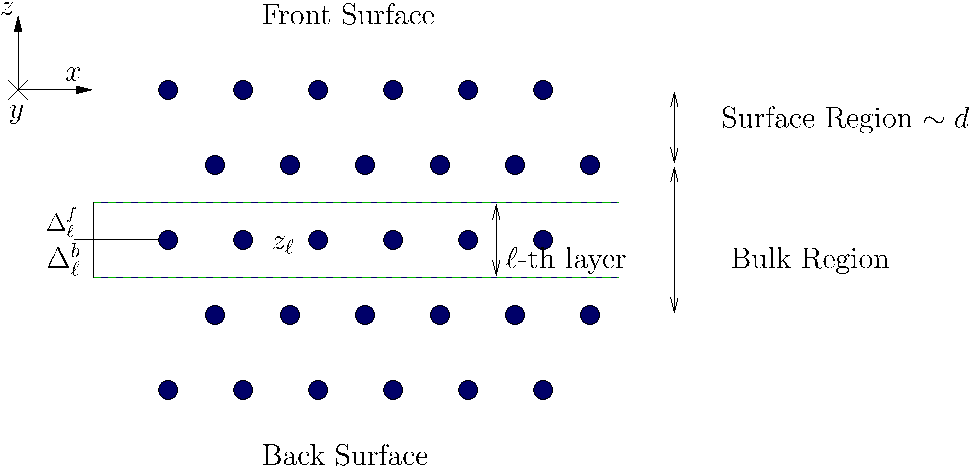
\includegraphics[height=5cm,width=7cm]{slab}
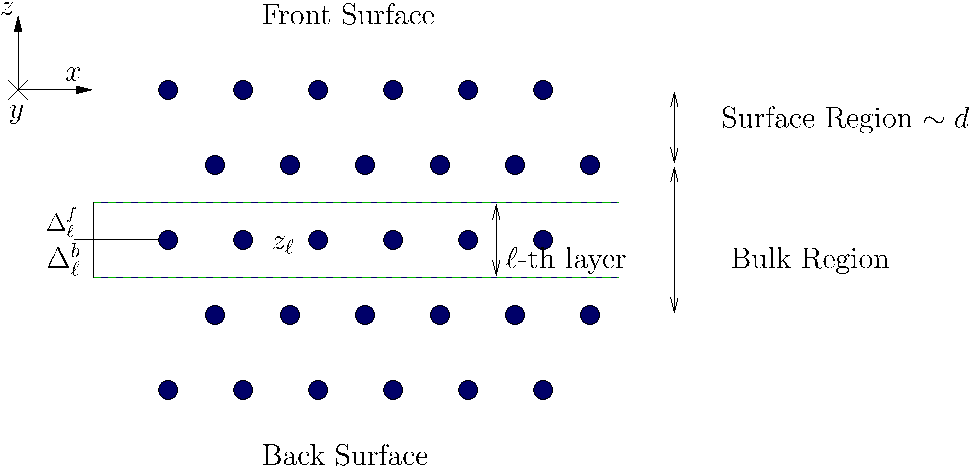
\includegraphics[scale=.7]{content/figures/diag-slab}
\caption{A sketch of a slab where the circles represent atoms.\label{fslab}}
\end{figure}

Now, we show how this ``cut function'' $\mathcal{C}^{\ell}(z)$ is introduced in
the calculation of $\chi_{\mathrm{abc}}$. 
The microscopic current density is given by
\begin{equation}\label{jmic}
\mathbf{j}(\mathbf{r},t)=\mathrm{Tr}(\hat{\mathbf{j}}(\mathbf{r})\hat{\rho}(t)),
\end{equation}
where the operator for the electron's current is
\begin{equation}\label{hatjmic}
\hat{\mathbf{j}}(\mathbf{r})=\frac{e}{2}\left(\hat{\mathbf{v}}^{\Sigma} |\mathbf{r}\rangle\langle\mathbf{r}|
+ |\mathbf{r}\rangle\langle\mathbf{r}|\hat{\mathbf{v}}^{\Sigma}\right), 
\end{equation}
where $\hat{\mathbf{v}}^{\Sigma}$ is the electron's velocity operator to be dealt
with below. We define
$\hat{\mu} \equiv |\mathbf{r}\rangle\langle\mathbf{r}|$ and use the cyclic invariance of
the trace to write
\begin{align}\label{jmic2}
\mathrm{Tr}(\hat{\mathbf{j}}(\mathbf{r})\hat{\rho}(t)
&= \mathrm{Tr}(\hat{\rho}(t)\hat{\mathbf{j}}(\mathbf{r}))
= \frac{e}{2}
\left(
  \mathrm{Tr}(\hat{\rho}\hat{\mathbf{v}}^{\Sigma}\hat{\mu})
+ \mathrm{Tr}(\hat{\rho}\hat{\mu}\hat{\mathbf{v}}^{\Sigma})
\right)\nonumber\\
&= \frac{e}{2}\sum_{n\mathbf{k}}
\left(
\langle n\mathbf{k}| \hat{\rho}\hat{\mathbf{v}}^{\Sigma}\hat{\mu} |n\mathbf{k}\rangle
+ \langle n\mathbf{k}| \hat{\rho}\hat{\mu}\hat{\mathbf{v}}^{\Sigma} |n\mathbf{k}\rangle
\right)\nonumber\\
&= \frac{e}{2}\sum_{nm\mathbf{k}}\langle n\mathbf{k}|\hat{\rho} |m\mathbf{k}\rangle
\left(
\langle m\mathbf{k}| \hat{\mathbf{v}}^{\Sigma}|\mathbf{r}\rangle \langle\mathbf{r}|n\mathbf{k}\rangle
+ \langle m\mathbf{k}|\mathbf{r}\rangle \langle\mathbf{r}| \hat{\mathbf{v}}^{\Sigma} |n\mathbf{k}\rangle
\right)
\nonumber\\
\mathbf{j}(\mathbf{r},t)
&= \sum_{nm\mathbf{k}}\rho_{nm}(\mathbf{k};t)\mathbf{j}_{mn}(\mathbf{k};\mathbf{r}),
\end{align}
where
\begin{equation}\label{jmic3}
\mathbf{j}_{mn}(\mathbf{k};\mathbf{r})=
\frac{e}{2}
\left(
\langle m\mathbf{k}| \hat{\mathbf{v}}^{\Sigma} |\mathbf{r}\rangle \langle\mathbf{r}|n\mathbf{k}\rangle
+
\langle m\mathbf{k}|\mathbf{r}\rangle \langle\mathbf{r}| \hat{\mathbf{v}}^{\Sigma} |n\mathbf{k}\rangle
\right),
\end{equation}
are the matrix elements of the microscopic current operator,
and we have used the fact that the matrix elements between states $|n\mathbf{k}\rangle$
are diagonal in $\mathbf{k}$, i.e. proportional to $\delta(\mathbf{k}-\mathbf{k}')$.

Integrating the microscopic current $\mathbf{j}(\mathbf{r},t)$ over
the entire slab gives the averaged microscopic current density. 
If we want the contribution from only one region of the unit cell 
towards the total current, we can integrate $\mathbf{j}({\mathbf r},t)$ 
over the desired region. The contribution to the current density from the
$\ell$-th layer of the slab is given by
\begin{equation}\label{jsz}
\frac{1}{\Omega}\int d^3r\, \mathcal{C}^{\ell}(z)\, \mathbf{j}(\mathbf{r},t)
 \equiv \mathbf{J}^{\ell}(t),
\end{equation}
where $\mathbf{J}^{\ell}(t)$ is the microscopic current in the
$\ell$-th layer.
Therefore we define
\begin{equation}\label{vcal}
e{\boldsymbol{\mathcal{V}}}^{\Sigma,\ell}_{mn}(\mathbf{k})
\equiv
%\frac{1}{\Omega}
\int d^3r\, \mathcal{C}^{\ell}(z)\,\mathbf{j}_{mn}({\mathbf{k}};\mathbf{r}),
\end{equation}
to write
\begin{equation}\label{jmac}
J_a^{(N,\ell)}(t)=\frac{e}{\Omega}
\sum_{mn\mathbf{k}}
\mathcal{V}^{\Sigma,a,\ell}_{mn}(\mathbf{k})
\rho^{(N)}_{nm}(\mathbf{k};t),
\end{equation}
as the induced microscopic current of the $\ell$-th layer, to order $N$ 
in the external perturbation. The matrix elements of the 
density operator for $N=1,2$ are given by Eqs. \eqref{rho1} and
\eqref{rho2} respectively. 
The Fourier component of microscopic current of Eq. \eqref{jmac} is given by
\begin{equation}\label{jmac2}
J_{\mathrm{a}}^{(N,\ell)}(\omega_3)=\frac{e}{\Omega}
\sum_{mn\mathbf{k}}
\mathcal{V}^{\Sigma,\mathrm{a},\ell}_{mn}(\mathbf{k})
\rho^{(N)}_{nm}(\mathbf{k};\omega_3)
.
\end{equation}
We proceed to give an explicit expression of
$\boldsymbol{\mathcal{V}}^{\Sigma,\ell}_{mn}(\mathbf{k})$.
From
Eqs. \eqref{vcal} and \eqref{jmic3} we obtain
\begin{equation}\label{intj}
{\boldsymbol{\mathcal{V}}}^{\Sigma,\ell}_{mn}({\mathbf k})=
\frac{1}{2}
\int \mathrm{d}^3 r\,
 \mathcal{C}^{\ell}(z)
\bigg[
\langle m\mathbf{k}|\mathbf{v}^\Sigma | \mathbf{r}\rangle
\langle \mathbf{r} | n \mathbf k \rangle +
\langle m\mathbf{k} | \mathbf{r}\rangle
\langle \mathbf{r} | \mathbf{v}^\Sigma | n \mathbf k \rangle\bigg]
,
\end{equation}  
and using the following property
\begin{equation}\label{nl.2}
\langle \mathbf{r} | \hat{\mathbf{v}}^{\Sigma}(\mathbf{r},\mathbf{r}')| n\mathbf{k} \rangle
=\int d^3 r'' \langle\mathbf{r}|\hat{\mathbf{v}}^{\Sigma}(\mathbf{r},\mathbf{r}')|\mathbf{r}''\rangle
\langle\mathbf{r}''|n\mathbf{k}\rangle
=\hat{\mathbf{v}}^{\Sigma}(\mathbf{r},\mathbf{r}'')
\int d^3 r'' \langle\mathbf{r}|\mathbf{r}''\rangle
\langle\mathbf{r}''|n\mathbf{k}\rangle
=\hat{\mathbf{v}}^{\Sigma}(\mathbf{r},\mathbf{r}')
\psi_{n\mathbf{k}}(\mathbf{r})
,
\end{equation}
that stems from the fact that the operator $\mathbf{v}^\Sigma(\mathbf{r},\mathbf{r}')$ does not act on
$\mathbf{r}''$, we can write
\begin{align}\label{nl.3}
\boldsymbol{\mathcal{V}}^{\Sigma,\ell}_{mn}({\mathbf k})
&=
\frac{1}{2}
\int \mathrm{d}^3 r\,
 \mathcal{C}^{\ell}(z)
 \bigg[
\psi_{n\mathbf{k}}(\mathbf{r})
\hat{\mathbf{v}}^{\Sigma *}\psi^{*}_{m\mathbf{k}}(\mathbf{r})
+ 
\psi^*_{m\mathbf{k}}(\mathbf{r})\hat{\mathbf{v}}^{\Sigma}
\psi_{n\mathbf{k}}(\mathbf{r})
\bigg]
\nonumber\\
&=
\int \mathrm{d}^3 r\,
\psi^*_{m\mathbf{k}}(\mathbf{r})
\left[\frac{\mathcal{C}^{\ell}(z) \mathbf{v}^\Sigma +
\mathbf{v}^\Sigma \mathcal{C}^{\ell}(z)}{2}\right]
\psi_{n\mathbf{k}}(\mathbf{r})
\nonumber\\
&=
\int \mathrm{d}^3 r\,
\psi^*_{m\mathbf{k}}(\mathbf{r})
\boldsymbol{\mathcal{V}}^{\Sigma,\ell}
\psi_{n\mathbf{k}}(\mathbf{r})
.
\end{align}
We used the hermitian property of $\mathbf{v}^\Sigma$ and defined
\begin{align}\label{nl.4}
\boldsymbol{\mathcal{V}}^{\Sigma,\ell}
=
\frac{\mathcal{C}^{\ell}(z) \mathbf{v}^\Sigma +
\mathbf{v}^\Sigma \mathcal{C}^{\ell}(z)}{2}
,
\end{align} 
where the superscript $\ell$ is inherited from $\mathcal{C}^{\ell}(z)$ and we
supress the dependance on $z$ from the increasingly crowded notation.  
We see that the replacement
\begin{align}\label{vcali}
\hat{\mathbf{v}}^{\Sigma} \to \hat{\boldsymbol{\mathcal{V}}}^{\Sigma,\ell}=\left[\frac{\mathcal{C}^{\ell}(z) \hat{\mathbf{v}}^{\Sigma} +
\hat{\mathbf{v}}^{\Sigma}\mathcal{C}^{\ell}(z)}{2}\right]
,
\end{align} 
is all that is needed to change the
velocity operator of the electron $\hat{\mathbf{v}}^{\Sigma}$ to the new velocity
operator $\boldsymbol{\mathcal{V}}^{\Sigma,\ell}$ that implicitly takes into account the
contribution of the region of the slab given by $\mathcal{C}^{\ell}(z)$.
From Eq. \eqref{vop2},
\begin{align}\label{vopii}
\boldsymbol{\mathcal{V}}^{\Sigma,\ell}
&=
\boldsymbol{\mathcal{V}}^{\mathrm{LDA},\ell}
+
\boldsymbol{\mathcal{V}}^{\mathcal{S},\ell}
\nonumber\\
\boldsymbol{\mathcal{V}}^{\mathrm{LDA},\ell}
&=
\boldsymbol{\mathcal{V}}^{\ell}
+
\boldsymbol{\mathcal{V}}^{\mathrm{nl},\ell}
=
\frac{1}{m_{e}}
\boldsymbol{\mathcal{P}}^{\ell}
+
\boldsymbol{\mathcal{V}}^{\mathrm{nl},\ell}
.
\end{align}
We remark that the simple relationship between 
$\mathbf{v}^{\Sigma}_{nm}(\mathbf{k})$ 
and 
$\mathbf{v}^{\mathrm{LDA}}_{nm}(\mathbf{k})$,
given in 
Eq. \eqref{chon.9}, 
does not hold between
$\boldsymbol{\mathcal{V}}^{\Sigma,\ell}_{nm}(\mathbf{k})$   
and 
$\boldsymbol{\mathcal{V}}^{\mathrm{LDA},\ell}_{nm}(\mathbf{k})$,
i.e.
$\boldsymbol{\mathcal{V}}^{\Sigma,\ell}_{nm}(\mathbf{k})\ne
(\omega^\Sigma_{nm}/\omega_{nm})
\boldsymbol{\mathcal{V}}^{\mathrm{LDA},\ell}_{nm}(\mathbf{k})$ 
and
$\boldsymbol{\mathcal{V}}^{\Sigma,\ell}_{nn}(\mathbf{k})\ne
\boldsymbol{\mathcal{V}}^{\mathrm{LDA},\ell}_{nn}(\mathbf{k})$
,
and thus, to calculate
$\boldsymbol{\mathcal{V}}^{\Sigma,\ell}_{nm}(\mathbf{k})$ 
we must calculate the matrix elements of $\boldsymbol{\mathcal{V}}^{\mathcal{S},\ell}$ and
$\boldsymbol{\mathcal{V}}^{\mathrm{LDA},\ell}$ (separately)
according to the expressions of
Appendix \ref{app:calvs}. {\color{red}Aeroport Charles de Gaulle, Nov. 30,
2014, see Appendix \ref{app:voila}}.
% Using Eq. \eqref{chon.9}, the matrix elements of Eq. \eqref{vcali}
% are given by
% \begin{align}\label{end.1}
% \boldsymbol{\mathcal{V}}^{\Sigma,\ell}_{nm}(\mathbf{k})
% &=
% \frac{1}{2}
% \sum_q
% \Big(
% \mathcal{C}^{\ell}_{nq}\mathbf{v}^\Sigma_{qm}
% +
% \mathbf{v}^\Sigma_{nq}\mathcal{C}^{\ell}_{qm}
% \Big)
% \nonumber\\
% &=
% \frac{1}{2}
% \Big(
% \mathcal{C}^{\ell}_{nn}\mathbf{v}^\Sigma_{nm}
% +
% \mathbf{v}^\Sigma_{nn}\mathcal{C}^{\ell}_{nm}
% +
% \mathcal{C}^{\ell}_{nm}\mathbf{v}^\Sigma_{mm}
% +
% \mathbf{v}^\Sigma_{nm}\mathcal{C}^{\ell}_{mm}
% \Big)
% \nonumber\\
% &+
% \frac{1}{2}
% \sum_{q\neq(nm)}
% \Big(
% \frac{\omega^\Sigma_{qm}}{\omega_{qm}}
% \mathcal{C}^{\ell}_{nq}\mathbf{v}^\mathrm{LDA}_{qm}
% +
% \frac{\omega^\Sigma_{nq}}{\omega_{nq}}
% \mathbf{v}^\mathrm{LDA}_{nq}\mathcal{C}^{\ell}_{qm}
% \Big)
% ,
% \end{align}
% \begin{align}\label{end.2}
% \boldsymbol{\mathcal{V}}^{\Sigma,\ell}_{nn}(\mathbf{k})
% &=
% \frac{1}{2}
% \Big(
% \mathcal{C}^{\ell}_{nn}\mathbf{v}^\Sigma_{nn}
% +
% \mathbf{v}^\Sigma_{nn}\mathcal{C}^{\ell}_{nn}
% \Big)
% \nonumber\\
% &+
% \frac{1}{2}
% \sum_{q\neq n}
% \Big(
% \frac{\omega^\Sigma_{qn}}{\omega_{qn}}
% \mathcal{C}^{\ell}_{nq}\mathbf{v}^\mathrm{LDA}_{qn}
% +
% \frac{\omega^\Sigma_{nq}}{\omega_{nq}}
% \mathbf{v}^\mathrm{LDA}_{nq}\mathcal{C}^{\ell}_{qn}
% \Big)
% \nonumber\\
% &=
% \mathcal{C}^{\ell}_{nn}\mathbf{v}^\mathrm{LDA}_{nn}
% \nonumber\\
% &+
% \frac{1}{2}
% \sum_{q\neq n}
% \frac{\omega^\Sigma_{qn}}{\omega_{qn}}
% \Big(
% \mathcal{C}^{\ell}_{nq}\mathbf{v}^\mathrm{LDA}_{qn}
% +
% \mathbf{v}^\mathrm{LDA}_{nq}\mathcal{C}^{\ell}_{qn}
% \Big)
% ,
% \end{align}

To limit the response to one surface, the equivalent of Eq. \eqref{nl.4} 
for $\boldsymbol{\mathcal{V}}^\ell=\boldsymbol{\mathcal{P}}^\ell/m_{e}$ was proposed in 
Ref. \cite{reiningPRB94} and later used in Refs.
\cite{mendozaPRL98},
\cite{mendozaPRB01},
\cite{sanoPRB02},
 and \cite{mejiaRMF04} 
also in the context of SHG. 
The layer-by-layer analysis of Refs. \cite{hoganPRB03} 
and \cite{castilloPRB03} used Eq. \eqref{sz}, 
limiting the current response
to a particular layer of the slab and used to obtain the
anisotropic linear optical response of semiconductor surfaces.
However, the first formal derivation of this scheme is presented in
Ref. \cite{mendozaPRB06} for the linear response, and here in this 
article, for the second harmonic optical response of semiconductors.


\section{Microscopic surface susceptibility}
In this section we obtain the expressions for the 
surface susceptibility tensor $\chi^S_{\mathrm{abc}}$.
We start with the basic relation $\mathbf{J} = d\mathbf{P}/dt$ 
with $\mathbf{J}$ the current calculated in Sec. \ref{cd}. From Eq. \eqref{jmac2} 
we obtain
\begin{equation}\label{Pjikn}
J_{\mathrm{a}}^{(2,\ell)}(2\omega)=-i2\tilde{\omega} P_{\mathrm{a}}(2\omega)
=\frac{e}{\Omega}
\sum_{mn\mathbf{k}}
\mathcal{V}^{\Sigma,\mathrm{a},\ell}_{mn}(\mathbf{k})
\rho^{(2)}_{nm}(\mathbf{k};2\omega)
,
\end{equation}
and using Eqs. \eqref{rho2} and \eqref{sshgp2} leads to
\begin{align}\label{Pjikn2}
\chi^{S,\ell}_{\mathrm{abc}}
&=
\frac{ie}{A E^{\mathrm{b}}_1E^{\mathrm{c}}_2 2\tilde{\omega}}
\sum_{mn\mathbf{k}}
\mathcal{V}^{\Sigma,\mathrm{a},\ell}_{mn}(\mathbf{k})
\rho^{(2)}_{nm}(\mathbf{k};2\tilde{\omega})
\nonumber \\
&=
\frac{e^2}{A\hbar2\tilde{\omega}}
\sum_{mn\mathbf{k}}
\frac{\mathcal{V}^{\Sigma,\mathrm{a},\ell}_{mn}(\mathbf{k})}
{\omega^\Sigma_{nm\mathbf{k}}-2\tilde{\omega}}
\bigg[
-(B_{nm}^{\mathrm{c}}(\mathbf{k},\omega))_{;k^{\mathrm{b}}}
\nonumber \\
&
+i\sum_\ell\left(r_{n\ell}^{\mathrm{b}}B_{\ell m}^{\mathrm{c}}(\mathbf{k},\omega) -
  B_{n\ell}^{\mathrm{c}}(\mathbf{k},\omega) 
  r_{\ell m}^{\mathrm{b}}\right)
\bigg]
,
\end{align}
which gives the surface-like susceptibility of $\ell$-th layer, where 
$\boldsymbol{\mathcal{V}}^\Sigma$ is given in Eq. \eqref{vopii},
where $A=\Omega/d$ is the surface area of the unit
cell that characterizes the surface of the system.
Using Eq. \eqref{rho1} we
split this equation into
two contributions from the first and second terms on the right hand side,
\begin{equation}\label{chii}
\chi_{i,\mathrm{abc}}^{S,\ell}
=-\frac{e^3}{A\hbar^22\tilde{\omega}}\sum_{mn\mathbf{k}}
\frac{\mathcal{V}_{mn}^{\Sigma,\mathrm{a},\ell}}{\omega^\Sigma_{nm}-2\tilde{\omega}}
\left(\frac{f_{mn}r_{nm}^{\mathrm{b}}}{\omega^\Sigma_{nm}-\tilde{\omega}}\right)_{;k^{\mathrm{c}}},
\end{equation} 
and 
\begin{equation}\label{chie}
\chi_{e,\mathrm{abc}}^{S,\ell}
=\frac{ie^3}{A\hbar^22\tilde{\omega}}\sum_{\ell mn\mathbf{k}}
\frac{\mathcal{V}_{mn}^{\Sigma,\mathrm{a},\ell}}{\omega^\Sigma_{nm}-2\tilde{\omega}}
\left(
\frac{r_{n\ell}^{\mathrm{c}} r_{\ell m}^{\mathrm{b}} 
f_{m\ell}}{\omega^\Sigma_{\ell m}-\tilde{\omega}}
-\frac{r_{n\ell}^{\mathrm{b}} r_{\ell m}^{\mathrm{c}} 
f_{\ell n}}{\omega^\Sigma_{n \ell}-\tilde{\omega}}
\right),
\end{equation} 
where $\boldsymbol{\chi}^{S,\ell}_i$
 is related to intraband transitions and
$\boldsymbol{\chi}^{S,\ell}_e$
to interband transitions.
For the generalized derivative in Eq. \eqref{chii} we use the chain rule 
\begin{equation}\label{gene2}
\left(\frac{f_{mn}r_{nm}^{\mathrm{b}}}{\omega^\Sigma_{nm}-\tilde{\omega}}\right)_{;k^{\mathrm{c}}}=
\frac{f_{mn}}{\omega^\Sigma_{nm}-\tilde{\omega}}\left(r_{nm}^{\mathrm{b}}\right)_{;k^{\mathrm{c}}}
-\frac{f_{mn}r_{nm}^{\mathrm{b}}\Delta_{nm}^\mathrm{c}}{(\omega^\Sigma_{nm}-\tilde{\omega})^2}
,
\end{equation}
and the following result
shown in Appendix \ref{app:gwk},
\begin{align}\label{eli.13}
\left(\omega^\Sigma_{nm}\right)_{;k^{\mathrm{a}}}
=
\left(\omega^{\mathrm{LDA}}_{nm}\right)_{;k^{\mathrm{a}}}
= 
v_{nn}^{\mathrm{LDA},\mathrm{a}}-v_{mm}^{\mathrm{LDA},\mathrm{a}}\equiv\Delta_{nm}^{\mathrm{a}}
.
\end{align} 

In order to calculate the nonlinear susceptibility of any given layer 
$\ell$ we simply add the above terms $\boldsymbol{\chi}^{S,\ell}=
\boldsymbol{\chi}_e^{S,\ell}+\boldsymbol{\chi}_i^{S,\ell}$ and 
then calculate the surface susceptibility as 
\begin{equation}\label{chiijksur}
\boldsymbol{\chi}^S\equiv \sum_{\ell=1}^{N}\boldsymbol{\chi}^{S,\ell},
\end{equation} 
where $\ell=1$ is the first layer right at the surface, 
and $\ell=N$ is the bulk-like layer (at a distance $\sim d$ from the
surface  as seen in
Fig. \ref{fsystem}), such that 
\begin{equation}\label{chiijksur2}
\boldsymbol{\chi}^{S,\ell=N}=0,
\end{equation}
in accordance to Eq. \eqref{sshg} valid for a centrosymmetric environment. 
We note that the value of
$N$ is not universal.
This means that the slab needs to have enough atomic layers for 
Eq. \eqref{chiijksur2} 
to be satisfied and to give converged results for $\boldsymbol{\chi}^S$. 
We can use Eq. \eqref{chiijksur} for
either the front or the back surface.

We can see from the prefactors of Eqs. \eqref{chii} and \eqref{chie} 
that they diverge as $\tilde{\omega}\to 0$. To remove this apparent divergence of 
$\boldsymbol{\chi}^{S,\ell}$, we perform a partial fraction expansion over $\tilde{\omega}$. 
As shown in Appendix \ref{appv}, we use time-reversal invariance to 
remove these divergences and obtain the following expressions for $\boldsymbol{\chi}^S$,
\begin{subequations}\label{eq:chis}
\begin{equation}
\mathrm{Im}[\chi^{\mathrm{a}\mathrm{b}\mathrm{c}}_{e,\omega}]= 
\frac{\pi |e|^3}{2\hbar^2}
\int \frac{d^{3}k}{8\pi^3}
\sum_{vc}\sum_{q\neq(v,c)}\frac{1}{\omega^\Sigma_{cv}}
\left[
\frac{\mathrm{Im}[\mathcal{V}^{\Sigma,\mathrm{a}}_{qc}\{r^{\mathrm{b}}_{cv}r^{\mathrm{c}}_{vq}\}]}
{(2\omega^\Sigma_{cv}-\omega^\Sigma_{cq})} 
-\frac{\mathrm{Im}[\mathcal{V}^{\Sigma,\mathrm{a}}_{vq}\{r^{\mathrm{c}}_{qc}r^{\mathrm{b}}_{cv}\}]}
{(2\omega^\Sigma_{cv}-\omega^\Sigma_{qv})}
\right]\delta(\omega^\Sigma_{cv}-\omega),
\end{equation}  
\begin{equation}
\mathrm{Im}[\chi^{\mathrm{a}\mathrm{b}\mathrm{c}}_{i,\omega}]= 
\frac{\pi\vert e\vert^3}{2\hbar^2}
\int \frac{d^{3}k}{8\pi^3}
\sum_{cv}\frac{1}{(\omega^\Sigma_{cv})^{2}}
\left[
\mathrm{Re}\left[\left\{r^{\mathrm{b}}_{cv}\left(\mathcal{V}^{\Sigma,\mathrm{a}}_{vc}\right)_{;k^{\mathrm{c}}}\right\}\right]
+\frac{\mathrm{Re}\left[\mathcal{V}^{\Sigma,\mathrm{a}}_{vc}\left\{r^{\mathrm{b}}_{cv}
\Delta^{\mathrm{c}}_{cv}\right\}\right]}{\omega^\Sigma_{cv}} 
\right]\delta(\omega^\Sigma_{cv}-\omega),
\end{equation}
\begin{equation}
\mathrm{Im}[\chi^{\mathrm{a}\mathrm{b}\mathrm{c}}_{e,2\omega}]= 
-\frac{\pi |e|^3}{2\hbar^2}
\int \frac{d^{3}k}{8\pi^3}
\sum_{vc}\frac{4}{\omega^\Sigma_{cv}}
\left[
\sum_{v'\ne
  v}\frac{\mathrm{Im}[\mathcal{V}^{\Sigma,\mathrm{a}}_{vc}\{r^{\mathrm{b}}_{cv'}r^{\mathrm{c}}_{v'v}\}]}
{2\omega^\Sigma_{cv'}-\omega^\Sigma_{cv}}
- \sum_{c'\ne
  c}\frac{\mathrm{Im}[\mathcal{V}^{\Sigma,\mathrm{a}}_{vc}\{r^{\mathrm{c}}_{cc'}r^{\mathrm{b}}_{c'v}\}]}
{2\omega^\Sigma_{c'v}-\omega^\Sigma_{cv}}
\right]\delta(\omega^\Sigma_{cv}-2\omega),
\end{equation}
\begin{equation}
\mathrm{Im}[\chi^{\mathrm{a}\mathrm{b}\mathrm{c}}_{i,2\omega}]= 
 \frac{\pi \vert
   e\vert^{3}}{2\hbar^2}
\int \frac{d^{3}k}{8\pi^3}
\sum_{vc}\frac{4}{(\omega^\Sigma_{cv})^{2}}
\left[\mathrm{Re}\left[\mathcal{V}^{\Sigma,\mathrm{a}}_{vc}\left\{\left(r^{\mathrm{b}}_{cv}\right)_{;k^{\mathrm{c}}}
\right\}\right] -
\frac{2\mathrm{Re}\left[\mathcal{V}^{\Sigma,\mathrm{a}}_{vc}\left\{r^{\mathrm{b}}_{cv}
\Delta^{\mathrm{c}}_{cv}\right\}\right]}{\omega^\Sigma_{cv}}\right]\delta(\omega^\Sigma_{cv}-2\omega)
,
\end{equation}
\end{subequations}
\noindent where the limit of $\eta\to 0$ has been taken.
We have split the interband and intraband $1\omega$ and $2\omega$
contributions. The real part of each contribution can be obtained through
a Kramers-Kronig transformation,\cite{nicolas} and then
$\chi^{S,\ell}_{\mathrm{abc}}=\chi^{S,\ell}_{e,\mathrm{abc},\omega} 
+\chi^{S,\ell}_{e,\mathrm{abc},2\omega}+\chi^{S,\ell}_{i,\mathrm{abc},\omega}
+\chi^{S,\ell}_{i,\mathrm{abc},2\omega}
$.
To fulfill the required intrinsic permutation symmetry,\cite{rashkeevPRB98} the
$\{\}$ notation symmetrizes the $\mathrm{b}\mathrm{c}$ Cartesian indices, i.e. $
\{u^{\mathrm{b}}s^{\mathrm{c}}\}=(u^{\mathrm{b}}s^{\mathrm{c}}+u^{\mathrm{c}}s^{
\mathrm{b}})/2$, and thus
$\chi_{\mathrm{abc}}^{S,\ell}=\chi_{\mathrm{a}\mathrm{c}\mathrm{b}}^{S,\ell}$.
In Appendices \ref{app:gdernl} and \ref{app:calvs} we demonstrate how to
calculate the generalized derivatives of $\mathbf{r}_{nm;\mathbf{k}}$ and
$\mathcal{V}^{\Sigma,\mathrm{a},\ell}_{nm;\mathbf{k}}$. We find that
\begin{align}\label{rgen.69}
(r^{\mathrm{b}}_{nm})_{;k^{\mathrm{a}}}
&=
-i\mathcal{T}^{\mathrm{a}\mathrm{b}}_{nm}
+
\frac{
r^{\mathrm{a}}_{nm}
\Delta^{\mathrm{b}}_{mn}
+r^{\mathrm{b}}_{nm}
\Delta^{\mathrm{a}}_{mn}
}
{\omega^{\mathrm{LDA}}_{nm}}
+
\frac{i}{\omega^{\mathrm{LDA}}_{nm}}
\sum_{\ell}
\bigg(
\omega^{\mathrm{LDA}}_{\ell m}
r^{\mathrm{a}}_{n\ell}
r^{\mathrm{b}}_{\ell m}
-
\omega^{\mathrm{LDA}}_{n\ell}
r^{\mathrm{b}}_{n\ell}
r^{\mathrm{a}}_{\ell m}
\bigg)
,
\end{align}
where
\begin{align}\label{tau.1}
\mathcal{T}_{nm}^{\mathrm{a}\mathrm{b}}
=
[r^{\mathrm{a}},v^{\mathrm{LDA},\mathrm{b}}]= 
\frac{i\hbar}{m_{e}}\delta_{ab}\delta_{nm} +
\mathcal{L}_{nm}^{\mathrm{a}\mathrm{b}}
,
\end{align}  
and
\begin{align}\label{tau.2}
\mathcal{L}_{nm}^{\mathrm{a}\mathrm{b}}
= \frac{1}{i\hbar}[r^{\mathrm{a}},v^{\mathrm{nl},\mathrm{b}}]_{nm}
,
\end{align}
is the contribution to the generalized derivative of $\mathbf{r}_{nm}$
coming from the nonlocal part of the pseudopotential.
In Appendix \ref{app:calt} we calculate
$\mathcal{L}^{\mathrm{a}\mathrm{b}}_{nm}$, that
is a term with very small numerical value but with a computational time 
at least an order of magnitude larger
than for all the other terms involved in the expressions for 
$\chi^{s,\ell}_{\mathrm{abc}}$.\cite{valerie}
Therefore, we neglect it throughout this article and take
\begin{align}\label{tau.69}
\mathcal{T}_{nm}^{\mathrm{a}\mathrm{b}}
\approx
\frac{i\hbar}{m_{e}}\delta_{ab}\delta_{nm}
.
\end{align} 
Finally,
we also need the following term (Eq. \eqref{ntita})
\begin{align}\label{a.3c}
(v^{\mathrm{LDA},\mathrm{a}}_{nn})_{;k^\mathrm{b}}
=
\nabla_{k^{\mathrm{a}}}  
v^{\mathrm{LDA},\mathrm{b}}_{nn}(\mathbf{k})
&=
-i\mathcal{T}^{\mathrm{a}\mathrm{b}}_{nn}
-
\sum_{\ell\ne n}
\omega^{\mathrm{LDA}}_{\ell n}
\bigg(  
r^{\mathrm{a}}_{n\ell}  
r^{\mathrm{b}}_{\ell n}
+  
r^{\mathrm{b}}_{n\ell}  
r^{\mathrm{a}}_{\ell n}
\bigg)
\nonumber\\
&\approx
\frac{\hbar}{m_{e}}\delta_{\mathrm{a}\mathrm{b}}
-
\sum_{\ell\ne n}
\omega^{\mathrm{LDA}}_{\ell n}
\bigg(  
r^{\mathrm{a}}_{n\ell}  
r^{\mathrm{b}}_{\ell n}
+  
r^{\mathrm{b}}_{n\ell}  
r^{\mathrm{a}}_{\ell n}
\bigg)
,
\end{align}  
among other quantities for $\mathcal{V}^{\Sigma,\mathrm{a},\ell}_{nm;\mathbf{k}}$, where we 
also use Eq. \eqref{tau.69}. Above is the standard effective-mas sum rule.
\cite{ashcroftbook} 
%In Appendix \ref{code}, we list all the quantities that should be
%coded in order to calculate the previous expressions for $\boldsymbol{\chi}$.

We have presented a complete derivation of the required elements to
calculate in the independent particle approach (IPA) the microscopic  
surface second harmonic susceptibility tensor $\boldsymbol{\chi}^S(-2\omega;\omega,\omega)$ 
using a layer-by-layer approach. We have done so for semiconductors using 
the length gauge for the coupling of the external electric field to the 
electron. 
%Also,
%we calculated the radiated efficiency $R$ within the three layer
%model. 
%The combination of $\boldsymbol{\chi}$ and $R$ allow us
%to study this fascinating surface optical phenomena.

\stopcontents[chapters]

